% 33-17(인쇄 33쪽) — 이항계수로 나타낸 파스칼의 삼각형 6단계까지와 색칠한 띠(₃C₃, ₄C₃, ₅C₃, ₆C₃ 를 잇는 비스듬한 띠).
% 스캔 화질이 낮아 TikZ 로 다시 그림. 색칠한 자리는 원문과 같고, 각 칸의 값(수)은 원문에도 없으므로 적지 않는다.
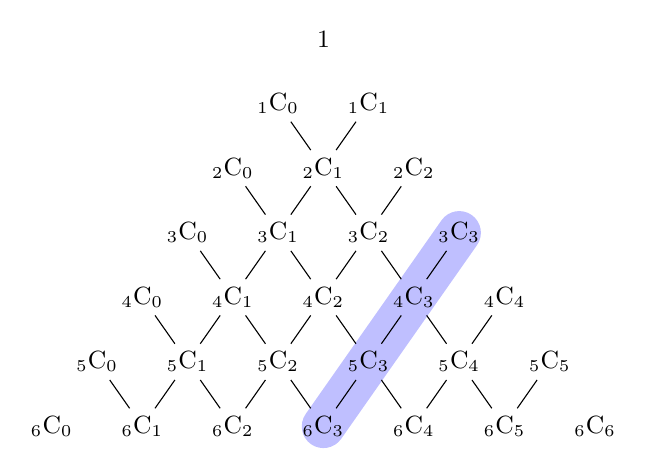
\begin{tikzpicture}[line width=0.4pt, font=\small,
  num/.style={inner sep=1.2pt},
  link/.style={line width=0.4pt, shorten >=8pt, shorten <=8pt}]
  % 행 k · 왼쪽부터 i 번째: x=(i-k/2)*1.15, y=-0.82k
  \coordinate (a00) at (0,0);
  \coordinate (a10) at (-0.575,-0.82); \coordinate (a11) at (0.575,-0.82);
  \coordinate (a20) at (-1.15,-1.64); \coordinate (a21) at (0,-1.64); \coordinate (a22) at (1.15,-1.64);
  \coordinate (a30) at (-1.725,-2.46); \coordinate (a31) at (-0.575,-2.46);
  \coordinate (a32) at (0.575,-2.46); \coordinate (a33) at (1.725,-2.46);
  \coordinate (a40) at (-2.3,-3.28); \coordinate (a41) at (-1.15,-3.28); \coordinate (a42) at (0,-3.28);
  \coordinate (a43) at (1.15,-3.28); \coordinate (a44) at (2.3,-3.28);
  \coordinate (a50) at (-2.875,-4.1); \coordinate (a51) at (-1.725,-4.1); \coordinate (a52) at (-0.575,-4.1);
  \coordinate (a53) at (0.575,-4.1); \coordinate (a54) at (1.725,-4.1); \coordinate (a55) at (2.875,-4.1);
  \coordinate (a60) at (-3.45,-4.92); \coordinate (a61) at (-2.3,-4.92); \coordinate (a62) at (-1.15,-4.92);
  \coordinate (a63) at (0,-4.92); \coordinate (a64) at (1.15,-4.92); \coordinate (a65) at (2.3,-4.92);
  \coordinate (a66) at (3.45,-4.92);
  % 색칠한 띠
  \draw[line width=5.5mm, blue!25, line cap=round] (a33) -- (a63);
  % 이웃하는 두 수를 아래 수에 잇는 짧은 선(가장자리에는 선이 없다 — 원문대로)
  \draw[link] (a10) -- (a21); \draw[link] (a11) -- (a21);
  \draw[link] (a20) -- (a31); \draw[link] (a21) -- (a31);
  \draw[link] (a21) -- (a32); \draw[link] (a22) -- (a32);
  \draw[link] (a30) -- (a41); \draw[link] (a31) -- (a41);
  \draw[link] (a31) -- (a42); \draw[link] (a32) -- (a42);
  \draw[link] (a32) -- (a43); \draw[link] (a33) -- (a43);
  \draw[link] (a40) -- (a51); \draw[link] (a41) -- (a51);
  \draw[link] (a41) -- (a52); \draw[link] (a42) -- (a52);
  \draw[link] (a42) -- (a53); \draw[link] (a43) -- (a53);
  \draw[link] (a43) -- (a54); \draw[link] (a44) -- (a54);
  \draw[link] (a50) -- (a61); \draw[link] (a51) -- (a61);
  \draw[link] (a51) -- (a62); \draw[link] (a52) -- (a62);
  \draw[link] (a52) -- (a63); \draw[link] (a53) -- (a63);
  \draw[link] (a53) -- (a64); \draw[link] (a54) -- (a64);
  \draw[link] (a54) -- (a65); \draw[link] (a55) -- (a65);
  \node[num] at (a00) {$1$};
  \node[num] at (a10) {${}_1\mathrm{C}_0$}; \node[num] at (a11) {${}_1\mathrm{C}_1$};
  \node[num] at (a20) {${}_2\mathrm{C}_0$}; \node[num] at (a21) {${}_2\mathrm{C}_1$}; \node[num] at (a22) {${}_2\mathrm{C}_2$};
  \node[num] at (a30) {${}_3\mathrm{C}_0$}; \node[num] at (a31) {${}_3\mathrm{C}_1$};
  \node[num] at (a32) {${}_3\mathrm{C}_2$}; \node[num] at (a33) {${}_3\mathrm{C}_3$};
  \node[num] at (a40) {${}_4\mathrm{C}_0$}; \node[num] at (a41) {${}_4\mathrm{C}_1$}; \node[num] at (a42) {${}_4\mathrm{C}_2$};
  \node[num] at (a43) {${}_4\mathrm{C}_3$}; \node[num] at (a44) {${}_4\mathrm{C}_4$};
  \node[num] at (a50) {${}_5\mathrm{C}_0$}; \node[num] at (a51) {${}_5\mathrm{C}_1$}; \node[num] at (a52) {${}_5\mathrm{C}_2$};
  \node[num] at (a53) {${}_5\mathrm{C}_3$}; \node[num] at (a54) {${}_5\mathrm{C}_4$}; \node[num] at (a55) {${}_5\mathrm{C}_5$};
  \node[num] at (a60) {${}_6\mathrm{C}_0$}; \node[num] at (a61) {${}_6\mathrm{C}_1$}; \node[num] at (a62) {${}_6\mathrm{C}_2$};
  \node[num] at (a63) {${}_6\mathrm{C}_3$}; \node[num] at (a64) {${}_6\mathrm{C}_4$}; \node[num] at (a65) {${}_6\mathrm{C}_5$};
  \node[num] at (a66) {${}_6\mathrm{C}_6$};
\end{tikzpicture}
